   \documentclass{article}
\usepackage{pgfplots}
\begin{document}
\begin{figure}
\centering

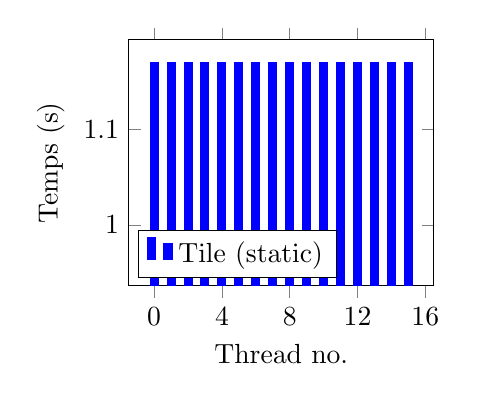
\begin{tikzpicture}
\begin{axis}[
  ybar,
  bar width=0.1cm,
  xlabel={Thread no.},
  ylabel={Temps (s)},
  ymin=.936264,
  legend pos=south west,
  width=0.45\textwidth,
  xtick distance=4
]

% Données pour le premier graphique (à gauche)
\addplot[color=blue, fill=blue] coordinates {
  (0,1.170388) (1,1.170330) (2,1.170388) (3,1.170402) (4,1.170333) (5,1.170350) (6,1.170352) (7,1.170367) (8,1.170345) (9,1.170392) (10,1.170345) (11,1.170379) (12,1.170406) (13,1.170388) (14,1.170386) (15,1.170338)
};
\addlegendentry{Tile (static)}

\end{axis}
\end{tikzpicture}
\hfill
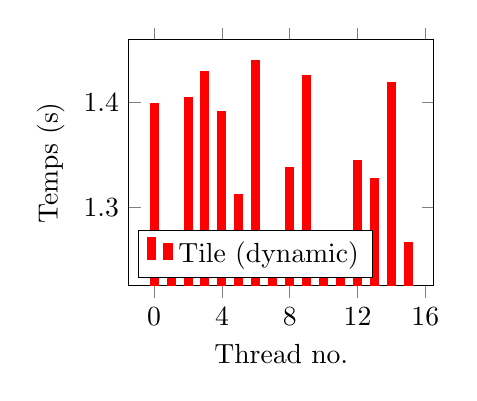
\begin{tikzpicture}
\begin{axis}[
  ybar,
  bar width=0.1cm,
  xlabel={Thread no.},
  ylabel={Temps (s)},
  ymin=,
  legend pos=south west,
  width=0.45\textwidth,
  xtick distance=4
]

% Données pour le deuxième graphique (au milieu)
\addplot[color=red, fill=red] coordinates {
  (0,1.398864) (1,1.271400) (2,1.404539) (3,1.429593) (4,1.391706) (5,1.311994) (6,1.440626) (7,1.258972) (8,1.337840) (9,1.425718) (10,1.244361) (11,1.248357) (12,1.344305) (13,1.327685) (14,1.419505) (15,1.266521)
};
\addlegendentry{Tile (dynamic)}

\end{axis}
\end{tikzpicture}
\hfill
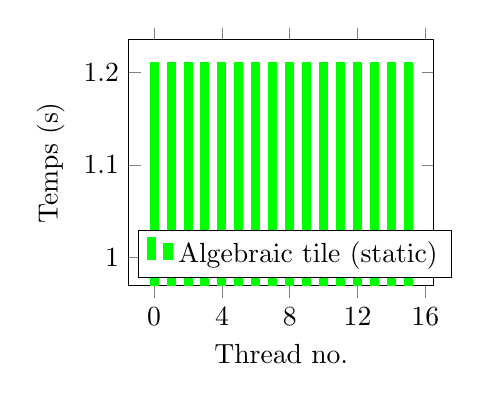
\begin{tikzpicture}
\begin{axis}[
  ybar,
  bar width=0.1cm,
  xlabel={Thread no.},
  ylabel={Temps (s)},
  ymin=.969005,
  legend pos=south west,
  width=0.45\textwidth,
  xtick distance=4
]

% Données pour le troisième graphique (à droite)
\addplot[color=green, fill=green] coordinates {
  (0,1.211327) (1,1.211364) (2,1.211257) (3,1.211338) (4,1.211286) (5,1.211326) (6,1.211279) (7,1.211303) (8,1.211298) (9,1.211325) (10,1.211348) (11,1.211334) (12,1.211287) (13,1.211265) (14,1.211376) (15,1.211359)
};
\addlegendentry{Algebraic tile (static)}

\end{axis}
\end{tikzpicture}

\caption{Temps d'exécution des threads pour le fichier gemm.c}
\label{fig:graphes}
\end{figure}

\begin{table}[htbp]
  \centering
  \caption{Statistiques pour le fichier gemm.c}
  \begin{tabular}{|c|c|c|c|}
    \hline
    Statistique & Algebraic Tile & Tile (static) & Tile (dynamic) \\ 
    \hline
    Skewness (g1) & -0.07076 & -0.0865338 & -0.116771 \\ 
    Kurtosis (g2) & -1.09266 & -1.4913 & -1.5185 \\ 
    Écart type & 3.49607e-05 & 2.50361e-05 & 0.0693181\\ 
    Percent Imbalance metric en \% & 0.00462306 & 0.00307595 & 7.10018\\ 
    Temps moyen (s) & 1.211376 & 1.170406 & 1.440626 \\ 
    \hline
  \end{tabular}
\end{table}
\newpage

\begin{figure}
\centering

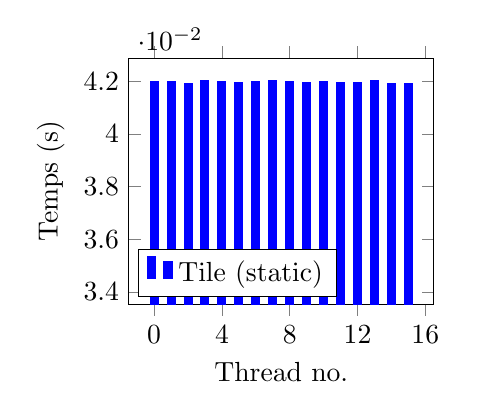
\begin{tikzpicture}
\begin{axis}[
  ybar,
  bar width=0.1cm,
  xlabel={Thread no.},
  ylabel={Temps (s)},
  ymin=.033535,
  legend pos=south west,
  width=0.45\textwidth,
  xtick distance=4
]

% Données pour le premier graphique (à gauche)
\addplot[color=blue, fill=blue] coordinates {
  (0,0.041999) (1,0.041994) (2,0.041919) (3,0.042024) (4,0.042007) (5,0.041935) (6,0.041991) (7,0.042009) (8,0.041993) (9,0.041944) (10,0.041996) (11,0.041934) (12,0.041966) (13,0.042029) (14,0.041923) (15,0.041932)
};
\addlegendentry{Tile (static)}

\end{axis}
\end{tikzpicture}
\hfill
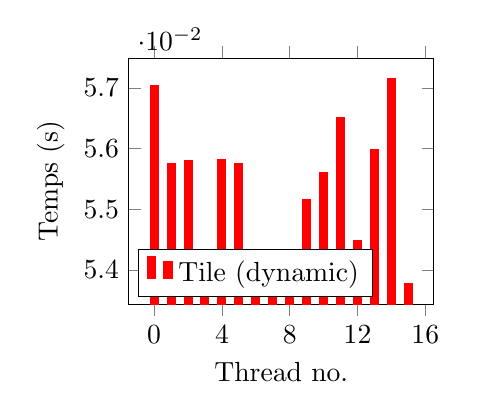
\begin{tikzpicture}
\begin{axis}[
  ybar,
  bar width=0.1cm,
  xlabel={Thread no.},
  ylabel={Temps (s)},
  ymin=,
  legend pos=south west,
  width=0.45\textwidth,
  xtick distance=4
]

% Données pour le deuxième graphique (au milieu)
\addplot[color=red, fill=red] coordinates {
  (0,0.057036) (1,0.055753) (2,0.055798) (3,0.054169) (4,0.055823) (5,0.055748) (6,0.053956) (7,0.053840) (8,0.054253) (9,0.055151) (10,0.055599) (11,0.056517) (12,0.054480) (13,0.055990) (14,0.057154) (15,0.053771)
};
\addlegendentry{Tile (dynamic)}

\end{axis}
\end{tikzpicture}
\hfill
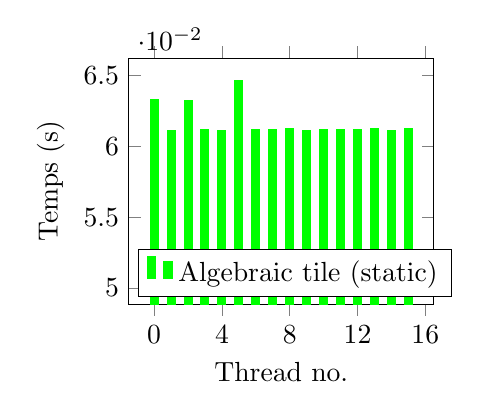
\begin{tikzpicture}
\begin{axis}[
  ybar,
  bar width=0.1cm,
  xlabel={Thread no.},
  ylabel={Temps (s)},
  ymin=.048863,
  legend pos=south west,
  width=0.45\textwidth,
  xtick distance=4
]

% Données pour le troisième graphique (à droite)
\addplot[color=green, fill=green] coordinates {
  (0,0.063279) (1,0.061131) (2,0.063215) (3,0.061159) (4,0.061079) (5,0.064631) (6,0.061197) (7,0.061152) (8,0.061228) (9,0.061129) (10,0.061153) (11,0.061203) (12,0.061196) (13,0.061256) (14,0.061118) (15,0.061209)
};
\addlegendentry{Algebraic tile (static)}

\end{axis}
\end{tikzpicture}

\caption{Temps d'exécution des threads pour le fichier gemver.c}
\label{fig:graphes}
\end{figure}

\begin{table}[htbp]
  \centering
  \caption{Statistiques pour le fichier gemver.c}
  \begin{tabular}{|c|c|c|c|}
    \hline
    Statistique & Algebraic Tile & Tile (static) & Tile (dynamic) \\ 
    \hline
    Skewness (g1) & 1.90217 & -0.193316 & 0.0546423 \\ 
    Kurtosis (g2) & 2.15588 & -1.46662 & -1.18217 \\ 
    Écart type & 0.0010312 & 3.66277e-05 & 0.00108303\\ 
    Percent Imbalance metric en \% & 4.84233 & 0.129364 & 3.32478\\ 
    Temps moyen (s) & 0.064631 & 0.042029 & 0.057154 \\ 
    \hline
  \end{tabular}
\end{table}
\newpage

\begin{figure}
\centering

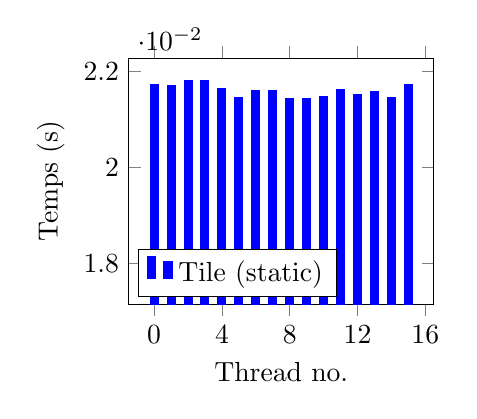
\begin{tikzpicture}
\begin{axis}[
  ybar,
  bar width=0.1cm,
  xlabel={Thread no.},
  ylabel={Temps (s)},
  ymin=.017144,
  legend pos=south west,
  width=0.45\textwidth,
  xtick distance=4
]

% Données pour le premier graphique (à gauche)
\addplot[color=blue, fill=blue] coordinates {
  (0,0.021733) (1,0.021704) (2,0.021805) (3,0.021812) (4,0.021644) (5,0.021464) (6,0.021606) (7,0.021600) (8,0.021430) (9,0.021445) (10,0.021471) (11,0.021626) (12,0.021516) (13,0.021591) (14,0.021453) (15,0.021730)
};
\addlegendentry{Tile (static)}

\end{axis}
\end{tikzpicture}
\hfill
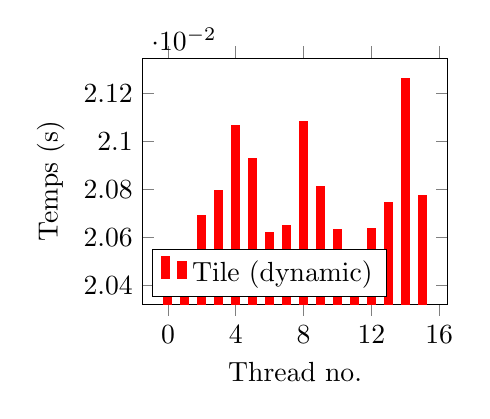
\begin{tikzpicture}
\begin{axis}[
  ybar,
  bar width=0.1cm,
  xlabel={Thread no.},
  ylabel={Temps (s)},
  ymin=,
  legend pos=south west,
  width=0.45\textwidth,
  xtick distance=4
]

% Données pour le deuxième graphique (au milieu)
\addplot[color=red, fill=red] coordinates {
  (0,0.020449) (1,0.020406) (2,0.020688) (3,0.020794) (4,0.021065) (5,0.020929) (6,0.020621) (7,0.020650) (8,0.021083) (9,0.020810) (10,0.020632) (11,0.020506) (12,0.020636) (13,0.020745) (14,0.021261) (15,0.020775)
};
\addlegendentry{Tile (dynamic)}

\end{axis}
\end{tikzpicture}
\hfill
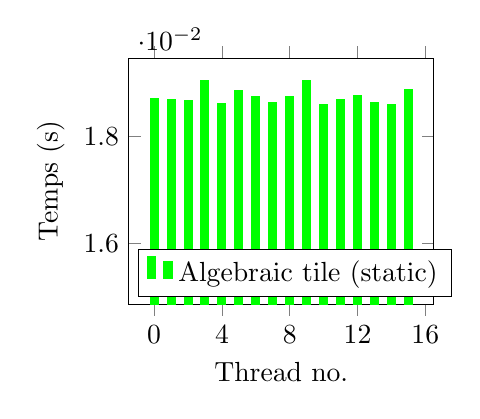
\begin{tikzpicture}
\begin{axis}[
  ybar,
  bar width=0.1cm,
  xlabel={Thread no.},
  ylabel={Temps (s)},
  ymin=.014872,
  legend pos=south west,
  width=0.45\textwidth,
  xtick distance=4
]

% Données pour le troisième graphique (à droite)
\addplot[color=green, fill=green] coordinates {
  (0,0.018715) (1,0.018690) (2,0.018673) (3,0.019044) (4,0.018613) (5,0.018858) (6,0.018752) (7,0.018636) (8,0.018747) (9,0.019048) (10,0.018591) (11,0.018694) (12,0.018758) (13,0.018643) (14,0.018594) (15,0.018874)
};
\addlegendentry{Algebraic tile (static)}

\end{axis}
\end{tikzpicture}

\caption{Temps d'exécution des threads pour le fichier gesummv.c}
\label{fig:graphes}
\end{figure}

\begin{table}[htbp]
  \centering
  \caption{Statistiques pour le fichier gesummv.c}
  \begin{tabular}{|c|c|c|c|}
    \hline
    Statistique & Algebraic Tile & Tile (static) & Tile (dynamic) \\ 
    \hline
    Skewness (g1) & 1.0517 & 0.172099 & 0.580779 \\ 
    Kurtosis (g2) & 0.092404 & -1.23117 & -0.328945 \\ 
    Écart type & 0.000138918 & 0.000125443 & 0.000228471\\ 
    Percent Imbalance metric en \% & 1.61318 & 0.9726 & 2.44735\\ 
    Temps moyen (s) & 0.019048 & 0.021812 & 0.021261 \\ 
    \hline
  \end{tabular}
\end{table}
\newpage

\begin{figure}
\centering

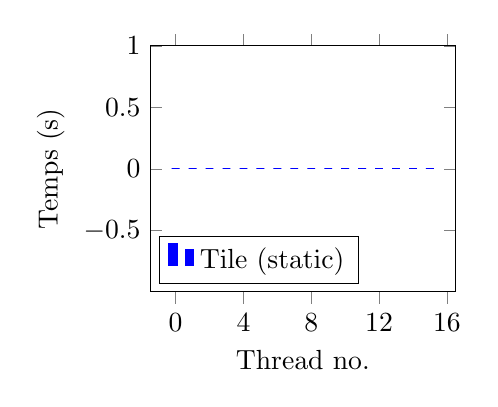
\begin{tikzpicture}
\begin{axis}[
  ybar,
  bar width=0.1cm,
  xlabel={Thread no.},
  ylabel={Temps (s)},
  ymin=0,
  legend pos=south west,
  width=0.45\textwidth,
  xtick distance=4
]

% Données pour le premier graphique (à gauche)
\addplot[color=blue, fill=blue] coordinates {
  (0,0.000000) (1,0.000000) (2,0.000000) (3,0.000000) (4,0.000000) (5,0.000000) (6,0.000000) (7,0.000000) (8,0.000000) (9,0.000000) (10,0.000000) (11,0.000000) (12,0.000000) (13,0.000000) (14,0.000000) (15,0.000000)
};
\addlegendentry{Tile (static)}

\end{axis}
\end{tikzpicture}
\hfill
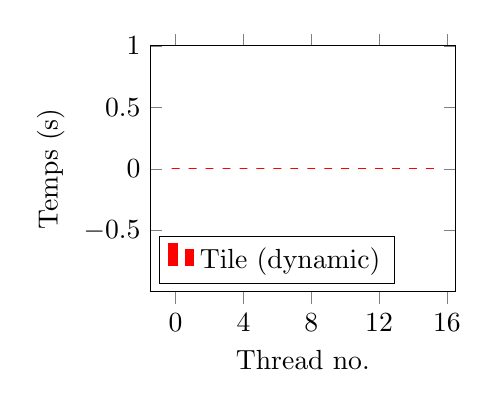
\begin{tikzpicture}
\begin{axis}[
  ybar,
  bar width=0.1cm,
  xlabel={Thread no.},
  ylabel={Temps (s)},
  ymin=,
  legend pos=south west,
  width=0.45\textwidth,
  xtick distance=4
]

% Données pour le deuxième graphique (au milieu)
\addplot[color=red, fill=red] coordinates {
  (0,0.000000) (1,0.000000) (2,0.000000) (3,0.000000) (4,0.000000) (5,0.000000) (6,0.000000) (7,0.000000) (8,0.000000) (9,0.000000) (10,0.000000) (11,0.000000) (12,0.000000) (13,0.000000) (14,0.000000) (15,0.000000)
};
\addlegendentry{Tile (dynamic)}

\end{axis}
\end{tikzpicture}
\hfill
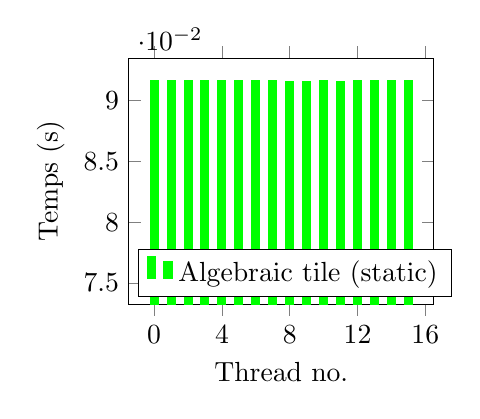
\begin{tikzpicture}
\begin{axis}[
  ybar,
  bar width=0.1cm,
  xlabel={Thread no.},
  ylabel={Temps (s)},
  ymin=.073260,
  legend pos=south west,
  width=0.45\textwidth,
  xtick distance=4
]

% Données pour le troisième graphique (à droite)
\addplot[color=green, fill=green] coordinates {
  (0,0.091630) (1,0.091623) (2,0.091623) (3,0.091630) (4,0.091590) (5,0.091615) (6,0.091585) (7,0.091590) (8,0.091575) (9,0.091575) (10,0.091605) (11,0.091582) (12,0.091605) (13,0.091615) (14,0.091620) (15,0.091620)
};
\addlegendentry{Algebraic tile (static)}

\end{axis}
\end{tikzpicture}

\caption{Temps d'exécution des threads pour le fichier symm.c}
\label{fig:graphes}
\end{figure}

\begin{table}[htbp]
  \centering
  \caption{Statistiques pour le fichier symm.c}
  \begin{tabular}{|c|c|c|c|}
    \hline
    Statistique & Algebraic Tile & Tile (static) & Tile (dynamic) \\ 
    \hline
    Skewness (g1) & -0.299759 &  &  \\ 
    Kurtosis (g2) & -1.39147 &  &  \\ 
    Écart type & 1.89183e-05 & 0 & 0\\ 
    Percent Imbalance metric en \% & 0.0270727 &  & \\ 
    Temps moyen (s) & 0.091630 & 0 & 0 \\ 
    \hline
  \end{tabular}
\end{table}
\newpage

\begin{figure}
\centering

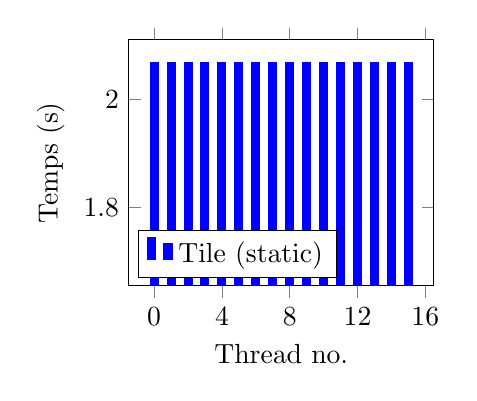
\begin{tikzpicture}
\begin{axis}[
  ybar,
  bar width=0.1cm,
  xlabel={Thread no.},
  ylabel={Temps (s)},
  ymin=1.655357,
  legend pos=south west,
  width=0.45\textwidth,
  xtick distance=4
]

% Données pour le premier graphique (à gauche)
\addplot[color=blue, fill=blue] coordinates {
  (0,2.069238) (1,2.069216) (2,2.069244) (3,2.069253) (4,2.069253) (5,2.069237) (6,2.069197) (7,2.069282) (8,2.069243) (9,2.069262) (10,2.069276) (11,2.069207) (12,2.069271) (13,2.069252) (14,2.069228) (15,2.069286)
};
\addlegendentry{Tile (static)}

\end{axis}
\end{tikzpicture}
\hfill
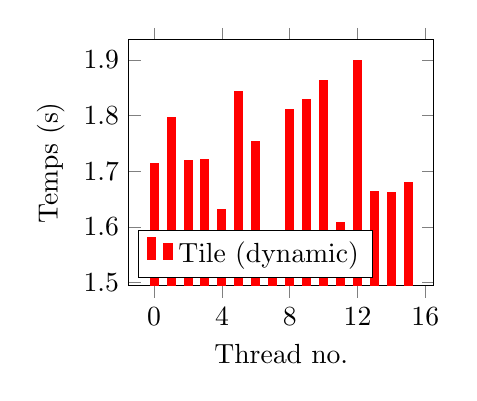
\begin{tikzpicture}
\begin{axis}[
  ybar,
  bar width=0.1cm,
  xlabel={Thread no.},
  ylabel={Temps (s)},
  ymin=,
  legend pos=south west,
  width=0.45\textwidth,
  xtick distance=4
]

% Données pour le deuxième graphique (au milieu)
\addplot[color=red, fill=red] coordinates {
  (0,1.714100) (1,1.796808) (2,1.719799) (3,1.721816) (4,1.631508) (5,1.842717) (6,1.753657) (7,1.531101) (8,1.810300) (9,1.829362) (10,1.863677) (11,1.607688) (12,1.899626) (13,1.662761) (14,1.661108) (15,1.679325)
};
\addlegendentry{Tile (dynamic)}

\end{axis}
\end{tikzpicture}
\hfill
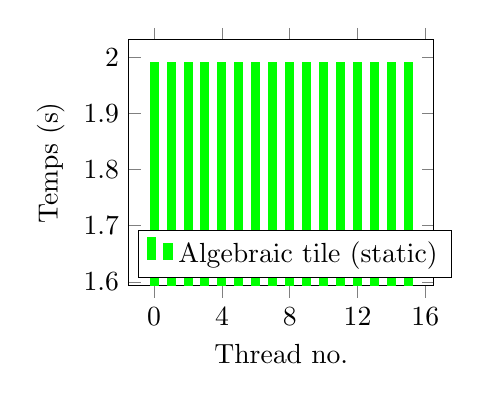
\begin{tikzpicture}
\begin{axis}[
  ybar,
  bar width=0.1cm,
  xlabel={Thread no.},
  ylabel={Temps (s)},
  ymin=1.593016,
  legend pos=south west,
  width=0.45\textwidth,
  xtick distance=4
]

% Données pour le troisième graphique (à droite)
\addplot[color=green, fill=green] coordinates {
  (0,1.991282) (1,1.991273) (2,1.991308) (3,1.991297) (4,1.991278) (5,1.991293) (6,1.991271) (7,1.991292) (8,1.991318) (9,1.991286) (10,1.991278) (11,1.991336) (12,1.991280) (13,1.991326) (14,1.991274) (15,1.991319)
};
\addlegendentry{Algebraic tile (static)}

\end{axis}
\end{tikzpicture}

\caption{Temps d'exécution des threads pour le fichier syr2k.c}
\label{fig:graphes}
\end{figure}

\begin{table}[htbp]
  \centering
  \caption{Statistiques pour le fichier syr2k.c}
  \begin{tabular}{|c|c|c|c|}
    \hline
    Statistique & Algebraic Tile & Tile (static) & Tile (dynamic) \\ 
    \hline
    Skewness (g1) & 0.674154 & -0.274896 & -0.144276 \\ 
    Kurtosis (g2) & -0.871847 & -0.7061 & -0.782305 \\ 
    Écart type & 2.01276e-05 & 2.5137e-05 & 0.0990718\\ 
    Percent Imbalance metric en \% & 0.00231006 & 0.00173976 & 9.62564\\ 
    Temps moyen (s) & 1.991336 & 2.069286 & 1.899626 \\ 
    \hline
  \end{tabular}
\end{table}
\newpage

\begin{figure}
\centering

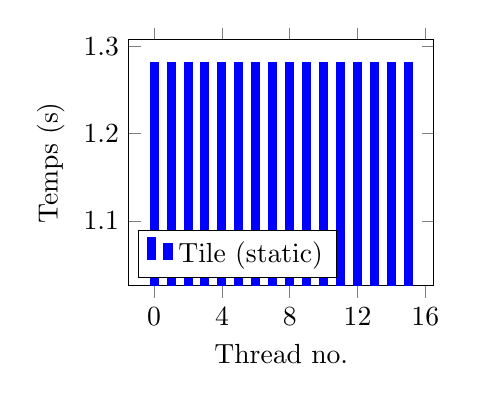
\begin{tikzpicture}
\begin{axis}[
  ybar,
  bar width=0.1cm,
  xlabel={Thread no.},
  ylabel={Temps (s)},
  ymin=1.025556,
  legend pos=south west,
  width=0.45\textwidth,
  xtick distance=4
]

% Données pour le premier graphique (à gauche)
\addplot[color=blue, fill=blue] coordinates {
  (0,1.281981) (1,1.281987) (2,1.281974) (3,1.282014) (4,1.281980) (5,1.281988) (6,1.281976) (7,1.282006) (8,1.281975) (9,1.282032) (10,1.282005) (11,1.281956) (12,1.282003) (13,1.281946) (14,1.282040) (15,1.282040)
};
\addlegendentry{Tile (static)}

\end{axis}
\end{tikzpicture}
\hfill
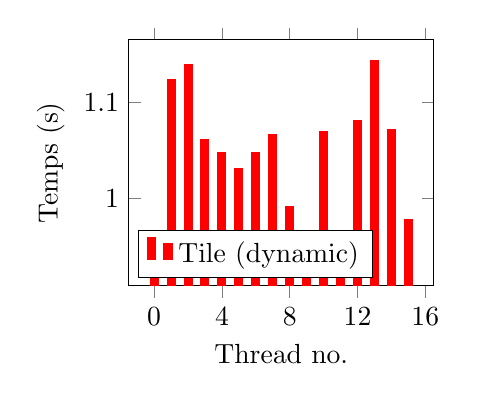
\begin{tikzpicture}
\begin{axis}[
  ybar,
  bar width=0.1cm,
  xlabel={Thread no.},
  ylabel={Temps (s)},
  ymin=,
  legend pos=south west,
  width=0.45\textwidth,
  xtick distance=4
]

% Données pour le deuxième graphique (au milieu)
\addplot[color=red, fill=red] coordinates {
  (0,0.941083) (1,1.124244) (2,1.139286) (3,1.061580) (4,1.048029) (5,1.030796) (6,1.048130) (7,1.066802) (8,0.990920) (9,0.930078) (10,1.069981) (11,0.935823) (12,1.081286) (13,1.143998) (14,1.071426) (15,0.977402)
};
\addlegendentry{Tile (dynamic)}

\end{axis}
\end{tikzpicture}
\hfill
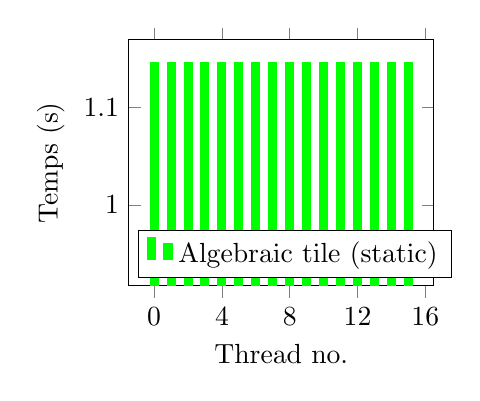
\begin{tikzpicture}
\begin{axis}[
  ybar,
  bar width=0.1cm,
  xlabel={Thread no.},
  ylabel={Temps (s)},
  ymin=.917000,
  legend pos=south west,
  width=0.45\textwidth,
  xtick distance=4
]

% Données pour le troisième graphique (à droite)
\addplot[color=green, fill=green] coordinates {
  (0,1.146250) (1,1.146318) (2,1.146300) (3,1.146328) (4,1.146305) (5,1.146295) (6,1.146302) (7,1.146346) (8,1.146300) (9,1.146294) (10,1.146276) (11,1.146295) (12,1.146277) (13,1.146277) (14,1.146345) (15,1.146333)
};
\addlegendentry{Algebraic tile (static)}

\end{axis}
\end{tikzpicture}

\caption{Temps d'exécution des threads pour le fichier syrk.c}
\label{fig:graphes}
\end{figure}

\begin{table}[htbp]
  \centering
  \caption{Statistiques pour le fichier syrk.c}
  \begin{tabular}{|c|c|c|c|}
    \hline
    Statistique & Algebraic Tile & Tile (static) & Tile (dynamic) \\ 
    \hline
    Skewness (g1) & 0.0292293 & 0.22702 & -0.252014 \\ 
    Kurtosis (g2) & -0.504821 & -0.767191 & -0.962259 \\ 
    Écart type & 2.55953e-05 & 2.70473e-05 & 0.06698\\ 
    Percent Imbalance metric en \% & 0.00401291 & 0.00390019 & 9.86248\\ 
    Temps moyen (s) & 1.146346 & 1.282040 & 1.143998 \\ 
    \hline
  \end{tabular}
\end{table}
\newpage

\begin{figure}
\centering

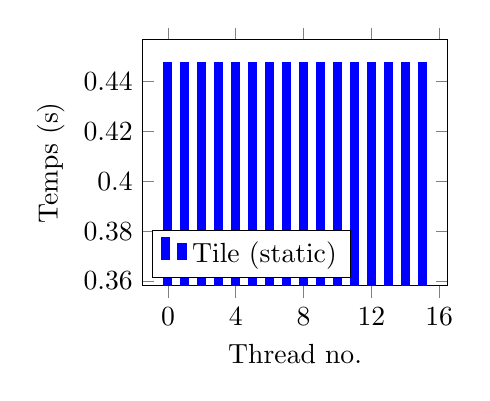
\begin{tikzpicture}
\begin{axis}[
  ybar,
  bar width=0.1cm,
  xlabel={Thread no.},
  ylabel={Temps (s)},
  ymin=.358045,
  legend pos=south west,
  width=0.45\textwidth,
  xtick distance=4
]

% Données pour le premier graphique (à gauche)
\addplot[color=blue, fill=blue] coordinates {
  (0,0.447884) (1,0.447620) (2,0.447576) (3,0.447614) (4,0.447648) (5,0.447608) (6,0.447619) (7,0.447600) (8,0.447569) (9,0.447609) (10,0.447588) (11,0.447557) (12,0.447568) (13,0.447620) (14,0.447610) (15,0.447656)
};
\addlegendentry{Tile (static)}

\end{axis}
\end{tikzpicture}
\hfill
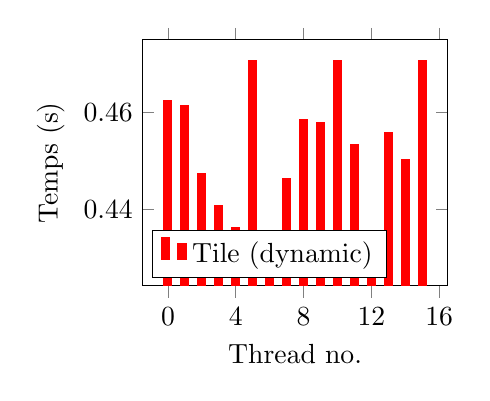
\begin{tikzpicture}
\begin{axis}[
  ybar,
  bar width=0.1cm,
  xlabel={Thread no.},
  ylabel={Temps (s)},
  ymin=,
  legend pos=south west,
  width=0.45\textwidth,
  xtick distance=4
]

% Données pour le deuxième graphique (au milieu)
\addplot[color=red, fill=red] coordinates {
  (0,0.462387) (1,0.461427) (2,0.447496) (3,0.440885) (4,0.436272) (5,0.470673) (6,0.429262) (7,0.446366) (8,0.458524) (9,0.457863) (10,0.470723) (11,0.453324) (12,0.428503) (13,0.455894) (14,0.450218) (15,0.470698)
};
\addlegendentry{Tile (dynamic)}

\end{axis}
\end{tikzpicture}
\hfill
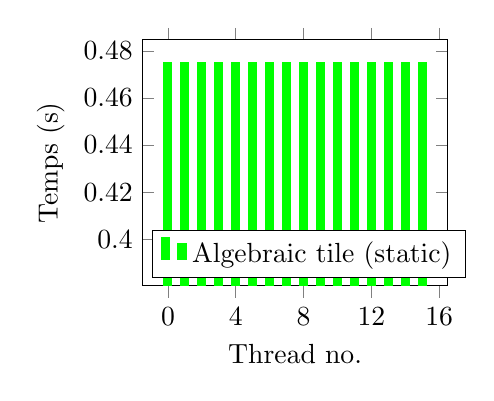
\begin{tikzpicture}
\begin{axis}[
  ybar,
  bar width=0.1cm,
  xlabel={Thread no.},
  ylabel={Temps (s)},
  ymin=.380146,
  legend pos=south west,
  width=0.45\textwidth,
  xtick distance=4
]

% Données pour le troisième graphique (à droite)
\addplot[color=green, fill=green] coordinates {
  (0,0.475250) (1,0.475218) (2,0.475260) (3,0.475221) (4,0.475231) (5,0.475207) (6,0.475228) (7,0.475214) (8,0.475246) (9,0.475238) (10,0.475213) (11,0.475223) (12,0.475276) (13,0.475183) (14,0.475265) (15,0.475195)
};
\addlegendentry{Algebraic tile (static)}

\end{axis}
\end{tikzpicture}

\caption{Temps d'exécution des threads pour le fichier trmm.c}
\label{fig:graphes}
\end{figure}

\begin{table}[htbp]
  \centering
  \caption{Statistiques pour le fichier trmm.c}
  \begin{tabular}{|c|c|c|c|}
    \hline
    Statistique & Algebraic Tile & Tile (static) & Tile (dynamic) \\ 
    \hline
    Skewness (g1) & 0.129257 & 2.82023 & -0.336844 \\ 
    Kurtosis (g2) & -0.652343 & 7.64351 & -0.879306 \\ 
    Écart type & 2.46716e-05 & 7.27881e-05 & 0.0132998\\ 
    Percent Imbalance metric en \% & 0.00988997 & 0.0585315 & 4.01983\\ 
    Temps moyen (s) & 0.475276 & 0.447884 & 0.470723 \\ 
    \hline
  \end{tabular}
\end{table}
\newpage

\begin{figure}
\centering

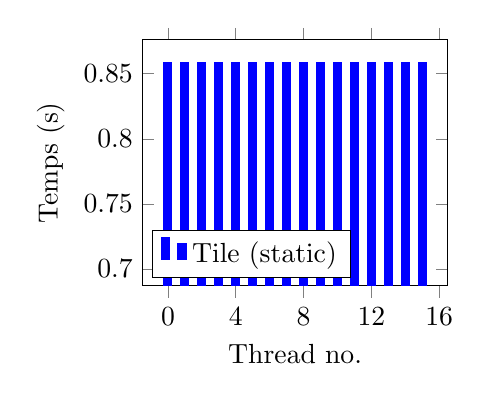
\begin{tikzpicture}
\begin{axis}[
  ybar,
  bar width=0.1cm,
  xlabel={Thread no.},
  ylabel={Temps (s)},
  ymin=.687056,
  legend pos=south west,
  width=0.45\textwidth,
  xtick distance=4
]

% Données pour le premier graphique (à gauche)
\addplot[color=blue, fill=blue] coordinates {
  (0,0.858872) (1,0.858871) (2,0.858900) (3,0.858821) (4,0.858879) (5,0.858894) (6,0.858897) (7,0.858859) (8,0.858876) (9,0.858890) (10,0.858913) (11,0.858834) (12,0.858867) (13,0.858899) (14,0.858903) (15,0.858864)
};
\addlegendentry{Tile (static)}

\end{axis}
\end{tikzpicture}
\hfill
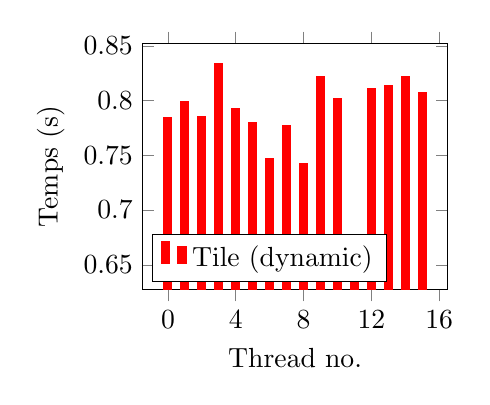
\begin{tikzpicture}
\begin{axis}[
  ybar,
  bar width=0.1cm,
  xlabel={Thread no.},
  ylabel={Temps (s)},
  ymin=,
  legend pos=south west,
  width=0.45\textwidth,
  xtick distance=4
]

% Données pour le deuxième graphique (au milieu)
\addplot[color=red, fill=red] coordinates {
  (0,0.784708) (1,0.799187) (2,0.785329) (3,0.833359) (4,0.792668) (5,0.779871) (6,0.746769) (7,0.776838) (8,0.742299) (9,0.822181) (10,0.802079) (11,0.646117) (12,0.810899) (13,0.813776) (14,0.821777) (15,0.807482)
};
\addlegendentry{Tile (dynamic)}

\end{axis}
\end{tikzpicture}
\hfill
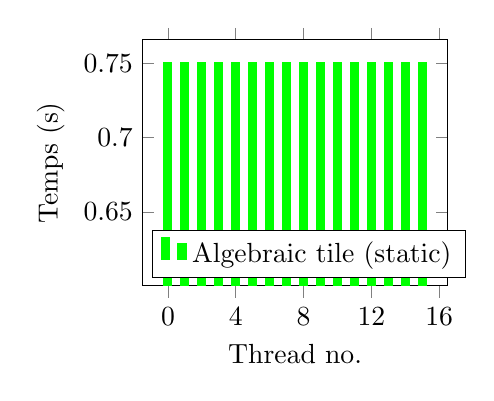
\begin{tikzpicture}
\begin{axis}[
  ybar,
  bar width=0.1cm,
  xlabel={Thread no.},
  ylabel={Temps (s)},
  ymin=.600452,
  legend pos=south west,
  width=0.45\textwidth,
  xtick distance=4
]

% Données pour le troisième graphique (à droite)
\addplot[color=green, fill=green] coordinates {
  (0,0.750656) (1,0.750591) (2,0.750605) (3,0.750658) (4,0.750635) (5,0.750566) (6,0.750670) (7,0.750638) (8,0.750689) (9,0.750644) (10,0.750585) (11,0.750681) (12,0.750694) (13,0.750581) (14,0.750677) (15,0.750709)
};
\addlegendentry{Algebraic tile (static)}

\end{axis}
\end{tikzpicture}

\caption{Temps d'exécution des threads pour le fichier 2mm.c}
\label{fig:graphes}
\end{figure}

\begin{table}[htbp]
  \centering
  \caption{Statistiques pour le fichier 2mm.c}
  \begin{tabular}{|c|c|c|c|}
    \hline
    Statistique & Algebraic Tile & Tile (static) & Tile (dynamic) \\ 
    \hline
    Skewness (g1) & -0.30406 & -0.756944 & -1.94848 \\ 
    Kurtosis (g2) & -1.17239 & -0.0441493 & 3.82799 \\ 
    Écart type & 4.34209e-05 & 2.43464e-05 & 0.0435132\\ 
    Percent Imbalance metric en \% & 0.00892569 & 0.00419152 & 6.11523\\ 
    Temps moyen (s) & 0.750709 & 0.858913 & 0.833359 \\ 
    \hline
  \end{tabular}
\end{table}
\newpage

\begin{figure}
\centering

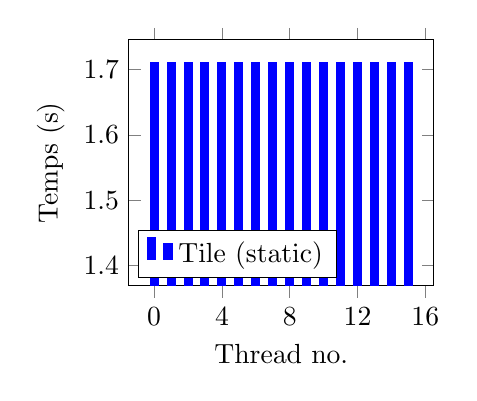
\begin{tikzpicture}
\begin{axis}[
  ybar,
  bar width=0.1cm,
  xlabel={Thread no.},
  ylabel={Temps (s)},
  ymin=1.368852,
  legend pos=south west,
  width=0.45\textwidth,
  xtick distance=4
]

% Données pour le premier graphique (à gauche)
\addplot[color=blue, fill=blue] coordinates {
  (0,1.711199) (1,1.711119) (2,1.711234) (3,1.711227) (4,1.711149) (5,1.711174) (6,1.711222) (7,1.711180) (8,1.711168) (9,1.711123) (10,1.711204) (11,1.711106) (12,1.711065) (13,1.711166) (14,1.711154) (15,1.711163)
};
\addlegendentry{Tile (static)}

\end{axis}
\end{tikzpicture}
\hfill
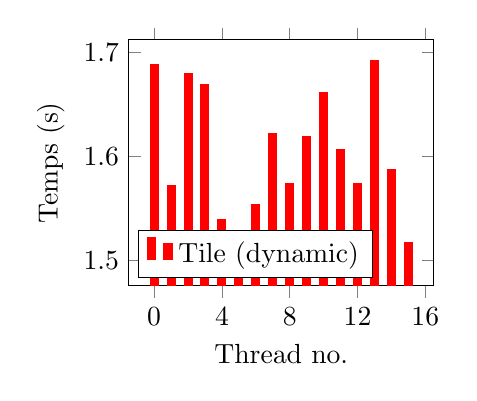
\begin{tikzpicture}
\begin{axis}[
  ybar,
  bar width=0.1cm,
  xlabel={Thread no.},
  ylabel={Temps (s)},
  ymin=,
  legend pos=south west,
  width=0.45\textwidth,
  xtick distance=4
]

% Données pour le deuxième graphique (au milieu)
\addplot[color=red, fill=red] coordinates {
  (0,1.688521) (1,1.571655) (2,1.679460) (3,1.668597) (4,1.539706) (5,1.495508) (6,1.553703) (7,1.621585) (8,1.573789) (9,1.618831) (10,1.661060) (11,1.606370) (12,1.574294) (13,1.692173) (14,1.587661) (15,1.517178)
};
\addlegendentry{Tile (dynamic)}

\end{axis}
\end{tikzpicture}
\hfill
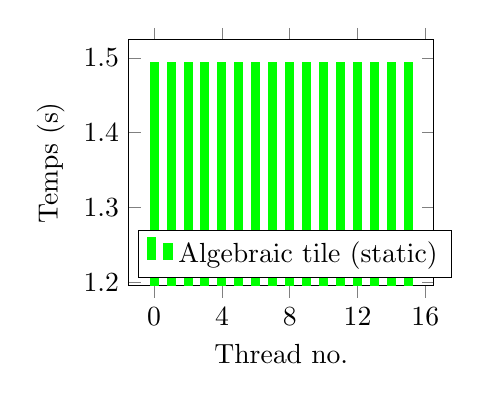
\begin{tikzpicture}
\begin{axis}[
  ybar,
  bar width=0.1cm,
  xlabel={Thread no.},
  ylabel={Temps (s)},
  ymin=1.195402,
  legend pos=south west,
  width=0.45\textwidth,
  xtick distance=4
]

% Données pour le troisième graphique (à droite)
\addplot[color=green, fill=green] coordinates {
  (0,1.494367) (1,1.494317) (2,1.494316) (3,1.494337) (4,1.494405) (5,1.494325) (6,1.494349) (7,1.494448) (8,1.494427) (9,1.494253) (10,1.494420) (11,1.494394) (12,1.494345) (13,1.494397) (14,1.494375) (15,1.494352)
};
\addlegendentry{Algebraic tile (static)}

\end{axis}
\end{tikzpicture}

\caption{Temps d'exécution des threads pour le fichier 3mm.c}
\label{fig:graphes}
\end{figure}

\begin{table}[htbp]
  \centering
  \caption{Statistiques pour le fichier 3mm.c}
  \begin{tabular}{|c|c|c|c|}
    \hline
    Statistique & Algebraic Tile & Tile (static) & Tile (dynamic) \\ 
    \hline
    Skewness (g1) & -0.295667 & -0.412821 & -0.0240204 \\ 
    Kurtosis (g2) & -0.245493 & -0.386939 & -1.10698 \\ 
    Écart type & 4.85891e-05 & 4.51237e-05 & 0.060023\\ 
    Percent Imbalance metric en \% & 0.00588881 & 0.00374013 & 5.55432\\ 
    Temps moyen (s) & 1.494448 & 1.711234 & 1.692173 \\ 
    \hline
  \end{tabular}
\end{table}
\newpage

\begin{figure}
\centering

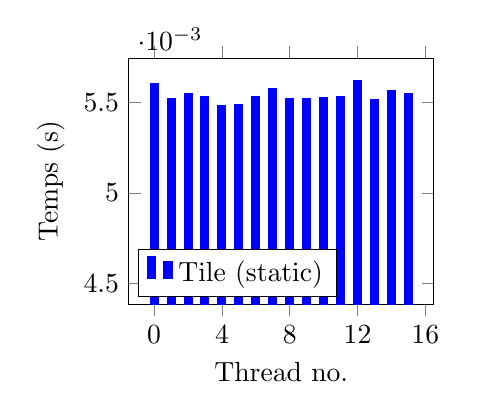
\begin{tikzpicture}
\begin{axis}[
  ybar,
  bar width=0.1cm,
  xlabel={Thread no.},
  ylabel={Temps (s)},
  ymin=.004386,
  legend pos=south west,
  width=0.45\textwidth,
  xtick distance=4
]

% Données pour le premier graphique (à gauche)
\addplot[color=blue, fill=blue] coordinates {
  (0,0.005604) (1,0.005520) (2,0.005551) (3,0.005534) (4,0.005483) (5,0.005489) (6,0.005535) (7,0.005579) (8,0.005524) (9,0.005520) (10,0.005528) (11,0.005530) (12,0.005621) (13,0.005515) (14,0.005568) (15,0.005549)
};
\addlegendentry{Tile (static)}

\end{axis}
\end{tikzpicture}
\hfill
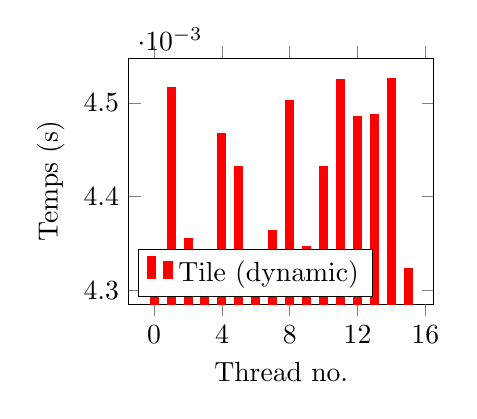
\begin{tikzpicture}
\begin{axis}[
  ybar,
  bar width=0.1cm,
  xlabel={Thread no.},
  ylabel={Temps (s)},
  ymin=,
  legend pos=south west,
  width=0.45\textwidth,
  xtick distance=4
]

% Données pour le deuxième graphique (au milieu)
\addplot[color=red, fill=red] coordinates {
  (0,0.004307) (1,0.004516) (2,0.004355) (3,0.004328) (4,0.004467) (5,0.004432) (6,0.004337) (7,0.004364) (8,0.004503) (9,0.004347) (10,0.004432) (11,0.004525) (12,0.004485) (13,0.004488) (14,0.004526) (15,0.004323)
};
\addlegendentry{Tile (dynamic)}

\end{axis}
\end{tikzpicture}
\hfill
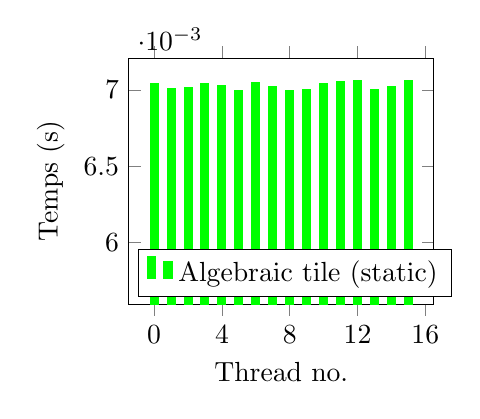
\begin{tikzpicture}
\begin{axis}[
  ybar,
  bar width=0.1cm,
  xlabel={Thread no.},
  ylabel={Temps (s)},
  ymin=.005597,
  legend pos=south west,
  width=0.45\textwidth,
  xtick distance=4
]

% Données pour le troisième graphique (à droite)
\addplot[color=green, fill=green] coordinates {
  (0,0.007039) (1,0.007012) (2,0.007014) (3,0.007044) (4,0.007032) (5,0.006997) (6,0.007050) (7,0.007023) (8,0.006999) (9,0.007002) (10,0.007042) (11,0.007057) (12,0.007061) (13,0.007005) (14,0.007024) (15,0.007062)
};
\addlegendentry{Algebraic tile (static)}

\end{axis}
\end{tikzpicture}

\caption{Temps d'exécution des threads pour le fichier atax.c}
\label{fig:graphes}
\end{figure}

\begin{table}[htbp]
  \centering
  \caption{Statistiques pour le fichier atax.c}
  \begin{tabular}{|c|c|c|c|}
    \hline
    Statistique & Algebraic Tile & Tile (static) & Tile (dynamic) \\ 
    \hline
    Skewness (g1) & 0.0361825 & 0.632402 & -0.0411392 \\ 
    Kurtosis (g2) & -1.3596 & -0.108419 & -1.63492 \\ 
    Écart type & 2.18588e-05 & 3.62231e-05 & 7.90249e-05\\ 
    Percent Imbalance metric en \% & 0.470341 & 1.45056 & 2.37642\\ 
    Temps moyen (s) & 0.007062 & 0.005621 & 0.004526 \\ 
    \hline
  \end{tabular}
\end{table}
\newpage

\begin{figure}
\centering

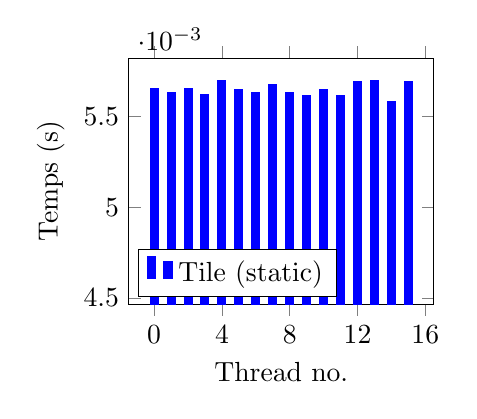
\begin{tikzpicture}
\begin{axis}[
  ybar,
  bar width=0.1cm,
  xlabel={Thread no.},
  ylabel={Temps (s)},
  ymin=.004465,
  legend pos=south west,
  width=0.45\textwidth,
  xtick distance=4
]

% Données pour le premier graphique (à gauche)
\addplot[color=blue, fill=blue] coordinates {
  (0,0.005656) (1,0.005631) (2,0.005656) (3,0.005623) (4,0.005695) (5,0.005647) (6,0.005629) (7,0.005673) (8,0.005629) (9,0.005615) (10,0.005649) (11,0.005617) (12,0.005690) (13,0.005698) (14,0.005582) (15,0.005693)
};
\addlegendentry{Tile (static)}

\end{axis}
\end{tikzpicture}
\hfill
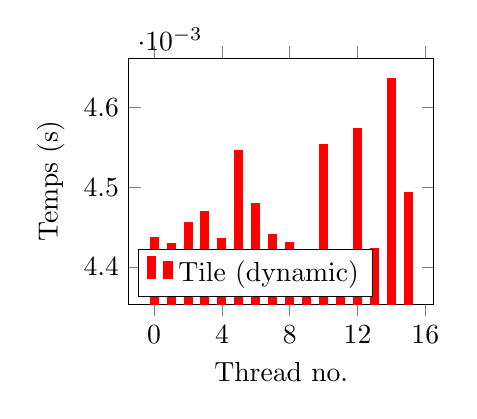
\begin{tikzpicture}
\begin{axis}[
  ybar,
  bar width=0.1cm,
  xlabel={Thread no.},
  ylabel={Temps (s)},
  ymin=,
  legend pos=south west,
  width=0.45\textwidth,
  xtick distance=4
]

% Données pour le deuxième graphique (au milieu)
\addplot[color=red, fill=red] coordinates {
  (0,0.004437) (1,0.004429) (2,0.004455) (3,0.004469) (4,0.004436) (5,0.004546) (6,0.004480) (7,0.004441) (8,0.004431) (9,0.004412) (10,0.004553) (11,0.004379) (12,0.004573) (13,0.004423) (14,0.004636) (15,0.004493)
};
\addlegendentry{Tile (dynamic)}

\end{axis}
\end{tikzpicture}
\hfill
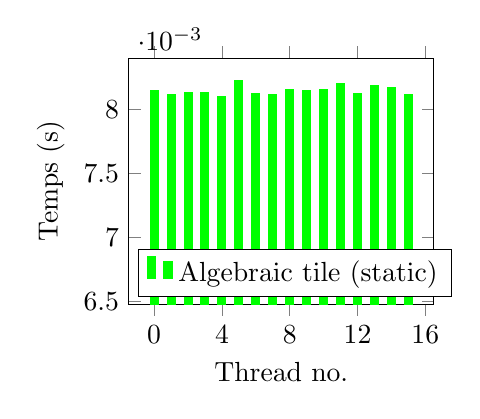
\begin{tikzpicture}
\begin{axis}[
  ybar,
  bar width=0.1cm,
  xlabel={Thread no.},
  ylabel={Temps (s)},
  ymin=.006481,
  legend pos=south west,
  width=0.45\textwidth,
  xtick distance=4
]

% Données pour le troisième graphique (à droite)
\addplot[color=green, fill=green] coordinates {
  (0,0.008147) (1,0.008119) (2,0.008130) (3,0.008129) (4,0.008102) (5,0.008226) (6,0.008122) (7,0.008117) (8,0.008159) (9,0.008147) (10,0.008152) (11,0.008206) (12,0.008122) (13,0.008183) (14,0.008168) (15,0.008119)
};
\addlegendentry{Algebraic tile (static)}

\end{axis}
\end{tikzpicture}

\caption{Temps d'exécution des threads pour le fichier bicg.c}
\label{fig:graphes}
\end{figure}

\begin{table}[htbp]
  \centering
  \caption{Statistiques pour le fichier bicg.c}
  \begin{tabular}{|c|c|c|c|}
    \hline
    Statistique & Algebraic Tile & Tile (static) & Tile (dynamic) \\ 
    \hline
    Skewness (g1) & 0.938244 & -0.0447433 & 0.926353 \\ 
    Kurtosis (g2) & -0.000188622 & -0.826671 & -0.00604333 \\ 
    Écart type & 3.35252e-05 & 3.28642e-05 & 6.68459e-05\\ 
    Percent Imbalance metric en \% & 0.972781 & 0.868482 & 3.60795\\ 
    Temps moyen (s) & 0.008226 & 0.005698 & 0.004636 \\ 
    \hline
  \end{tabular}
\end{table}
\newpage

\begin{figure}
\centering

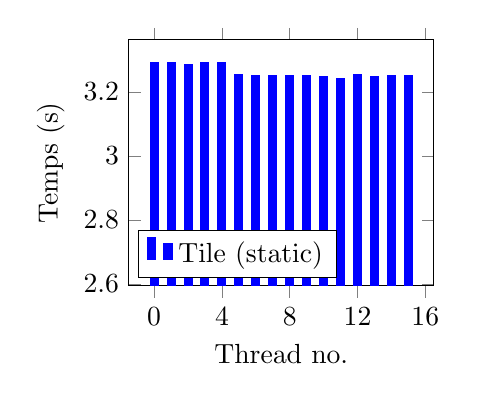
\begin{tikzpicture}
\begin{axis}[
  ybar,
  bar width=0.1cm,
  xlabel={Thread no.},
  ylabel={Temps (s)},
  ymin=2.594113,
  legend pos=south west,
  width=0.45\textwidth,
  xtick distance=4
]

% Données pour le premier graphique (à gauche)
\addplot[color=blue, fill=blue] coordinates {
  (0,3.292830) (1,3.292739) (2,3.285554) (3,3.290024) (4,3.290697) (5,3.252624) (6,3.250493) (7,3.249419) (8,3.250510) (9,3.250618) (10,3.246517) (11,3.242642) (12,3.252690) (13,3.247322) (14,3.249950) (15,3.252302)
};
\addlegendentry{Tile (static)}

\end{axis}
\end{tikzpicture}
\hfill
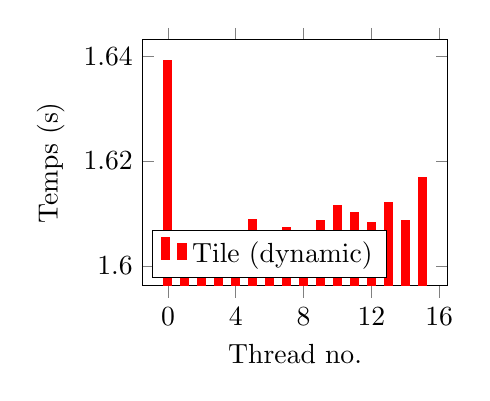
\begin{tikzpicture}
\begin{axis}[
  ybar,
  bar width=0.1cm,
  xlabel={Thread no.},
  ylabel={Temps (s)},
  ymin=,
  legend pos=south west,
  width=0.45\textwidth,
  xtick distance=4
]

% Données pour le deuxième graphique (au milieu)
\addplot[color=red, fill=red] coordinates {
  (0,1.639227) (1,1.606280) (2,1.605576) (3,1.604097) (4,1.602871) (5,1.608887) (6,1.600099) (7,1.607320) (8,1.605705) (9,1.608595) (10,1.611533) (11,1.610085) (12,1.608301) (13,1.612164) (14,1.608563) (15,1.616827)
};
\addlegendentry{Tile (dynamic)}

\end{axis}
\end{tikzpicture}
\hfill
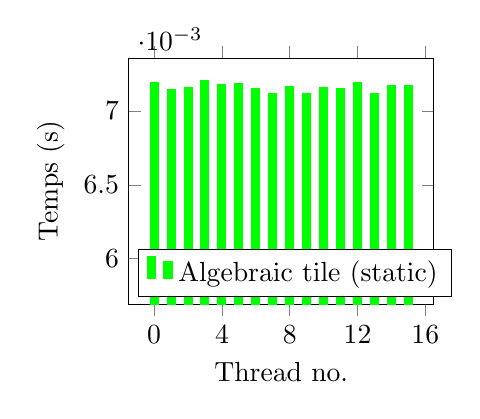
\begin{tikzpicture}
\begin{axis}[
  ybar,
  bar width=0.1cm,
  xlabel={Thread no.},
  ylabel={Temps (s)},
  ymin=.005692,
  legend pos=south west,
  width=0.45\textwidth,
  xtick distance=4
]

% Données pour le troisième graphique (à droite)
\addplot[color=green, fill=green] coordinates {
  (0,0.007193) (1,0.007144) (2,0.007156) (3,0.007206) (4,0.007178) (5,0.007182) (6,0.007151) (7,0.007120) (8,0.007166) (9,0.007116) (10,0.007160) (11,0.007150) (12,0.007192) (13,0.007119) (14,0.007170) (15,0.007174)
};
\addlegendentry{Algebraic tile (static)}

\end{axis}
\end{tikzpicture}

\caption{Temps d'exécution des threads pour le fichier doitgen.c}
\label{fig:graphes}
\end{figure}

\begin{table}[htbp]
  \centering
  \caption{Statistiques pour le fichier doitgen.c}
  \begin{tabular}{|c|c|c|c|}
    \hline
    Statistique & Algebraic Tile & Tile (static) & Tile (dynamic) \\ 
    \hline
    Skewness (g1) & -0.25121 & 0.774534 & 2.47238 \\ 
    Kurtosis (g2) & -0.819713 & -1.29322 & 6.18332 \\ 
    Écart type & 2.62452e-05 & 0.0191271 & 0.00850673\\ 
    Percent Imbalance metric en \% & 0.627561 & 0.935533 & 1.83052\\ 
    Temps moyen (s) & 0.007206 & 3.292830 & 1.639227 \\ 
    \hline
  \end{tabular}
\end{table}
\newpage

\begin{figure}
\centering

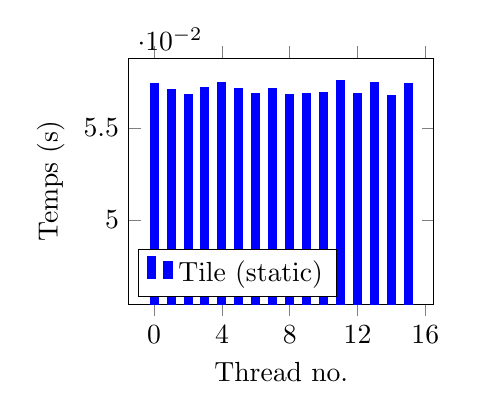
\begin{tikzpicture}
\begin{axis}[
  ybar,
  bar width=0.1cm,
  xlabel={Thread no.},
  ylabel={Temps (s)},
  ymin=.045432,
  legend pos=south west,
  width=0.45\textwidth,
  xtick distance=4
]

% Données pour le premier graphique (à gauche)
\addplot[color=blue, fill=blue] coordinates {
  (0,0.057411) (1,0.057067) (2,0.056844) (3,0.057181) (4,0.057449) (5,0.057160) (6,0.056871) (7,0.057129) (8,0.056821) (9,0.056857) (10,0.056921) (11,0.057582) (12,0.056899) (13,0.057469) (14,0.056791) (15,0.057429)
};
\addlegendentry{Tile (static)}

\end{axis}
\end{tikzpicture}
\hfill
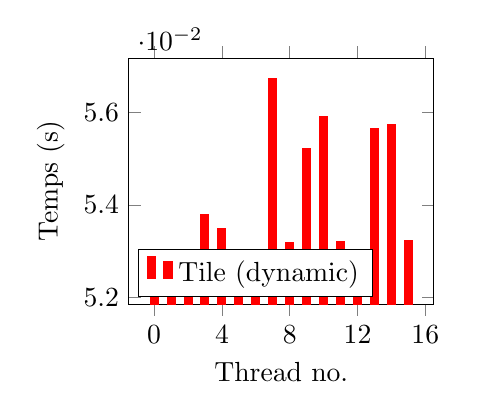
\begin{tikzpicture}
\begin{axis}[
  ybar,
  bar width=0.1cm,
  xlabel={Thread no.},
  ylabel={Temps (s)},
  ymin=,
  legend pos=south west,
  width=0.45\textwidth,
  xtick distance=4
]

% Données pour le deuxième graphique (au milieu)
\addplot[color=red, fill=red] coordinates {
  (0,0.052297) (1,0.052856) (2,0.052344) (3,0.053794) (4,0.053478) (5,0.052293) (6,0.052496) (7,0.056731) (8,0.053180) (9,0.055221) (10,0.055917) (11,0.053199) (12,0.052585) (13,0.055658) (14,0.055738) (15,0.053216)
};
\addlegendentry{Tile (dynamic)}

\end{axis}
\end{tikzpicture}
\hfill
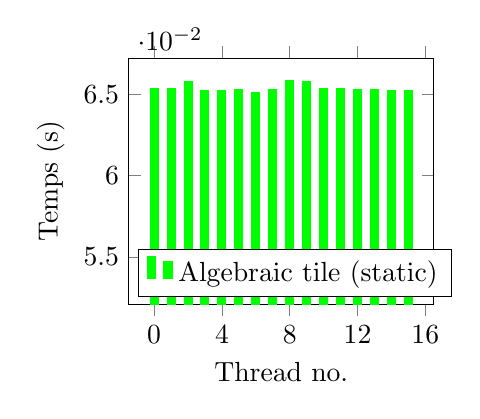
\begin{tikzpicture}
\begin{axis}[
  ybar,
  bar width=0.1cm,
  xlabel={Thread no.},
  ylabel={Temps (s)},
  ymin=.052101,
  legend pos=south west,
  width=0.45\textwidth,
  xtick distance=4
]

% Données pour le troisième graphique (à droite)
\addplot[color=green, fill=green] coordinates {
  (0,0.065336) (1,0.065321) (2,0.065804) (3,0.065219) (4,0.065250) (5,0.065312) (6,0.065127) (7,0.065282) (8,0.065845) (9,0.065772) (10,0.065325) (11,0.065342) (12,0.065273) (13,0.065309) (14,0.065204) (15,0.065220)
};
\addlegendentry{Algebraic tile (static)}

\end{axis}
\end{tikzpicture}

\caption{Temps d'exécution des threads pour le fichier mvt.c}
\label{fig:graphes}
\end{figure}

\begin{table}[htbp]
  \centering
  \caption{Statistiques pour le fichier mvt.c}
  \begin{tabular}{|c|c|c|c|}
    \hline
    Statistique & Algebraic Tile & Tile (static) & Tile (dynamic) \\ 
    \hline
    Skewness (g1) & 1.35533 & 0.347122 & 0.689487 \\ 
    Kurtosis (g2) & 0.306116 & -1.38889 & -1.0413 \\ 
    Écart type & 0.000216862 & 0.000265188 & 0.00146213\\ 
    Percent Imbalance metric en \% & 0.72463 & 0.813059 & 5.42307\\ 
    Temps moyen (s) & 0.065845 & 0.057582 & 0.056731 \\ 
    \hline
  \end{tabular}
\end{table}
\newpage

  \end{document}
